\documentclass[border=10pt]{standalone}
\usepackage[T1]{fontenc}
\usepackage{helvet}
\renewcommand{\familydefault}{\sfdefault}
\usepackage{tikz}
\usetikzlibrary{arrows.meta,positioning,calc,decorations.pathreplacing,fit}

\definecolor{idpblue}{HTML}{005DAA}
\definecolor{idpcyan}{HTML}{00B3FF}
\definecolor{warm}{HTML}{D7263D}
\definecolor{inkgray}{HTML}{444444}
\definecolor{forestgreen}{HTML}{2E7D32}

\begin{document}
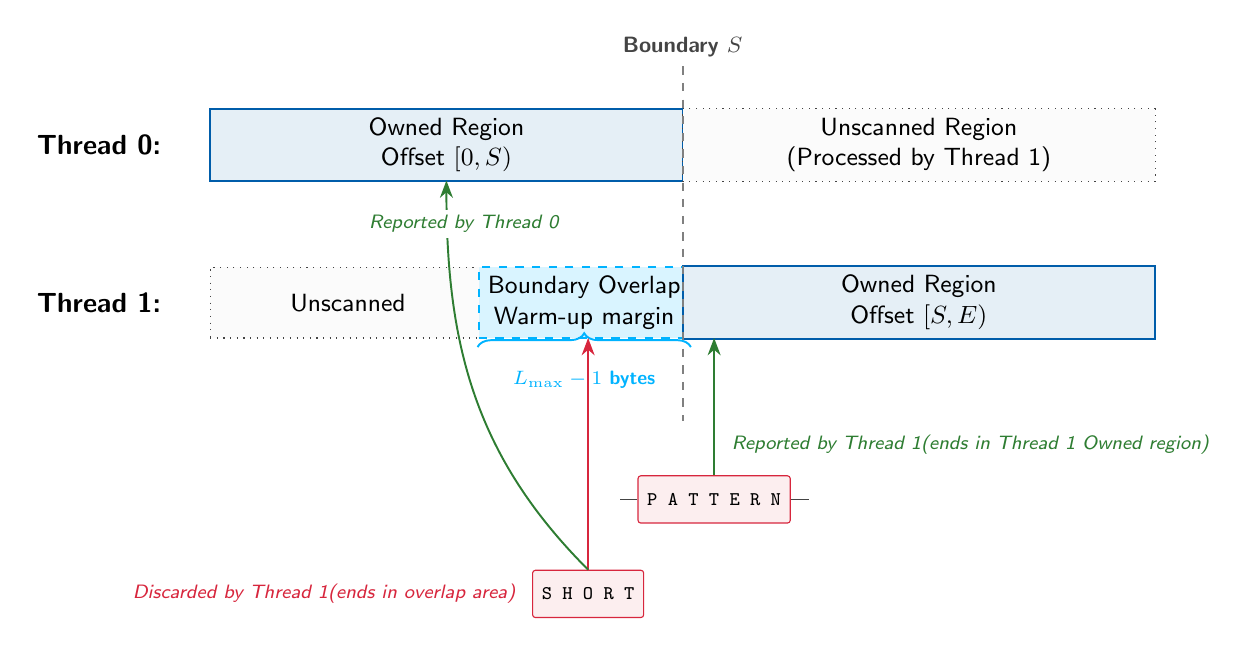
\begin{tikzpicture}[
    font=\small,
    >={Stealth[length=2.2mm]},
    bar/.style={draw=inkgray, minimum height=9mm, align=center, fill=gray!6},
    owned/.style={bar, fill=idpblue!10, draw=idpblue, line width=0.8pt},
    overlap/.style={bar, fill=idpcyan!15, draw=idpcyan, dashed, line width=0.8pt},
    pattern/.style={draw=warm, rounded corners=1pt, minimum height=6mm, fill=warm!8, font=\scriptsize\ttfamily},
    note/.style={font=\footnotesize, text=inkgray, align=center},
    label/.style={font=\bfseries},
]

    % --- Thread 0 Row ---
    \node[label, anchor=east] at (-0.5, 2.0) {Thread 0:};
    \node[owned, minimum width=60mm] (t0_owned) at (3.0, 2.0) {Owned Region\\Offset $[0, S)$};
    \node[bar, minimum width=60mm, fill=gray!3, dotted] (t0_rest) at (9.0, 2.0) {Unscanned Region\\(Processed by Thread 1)};

    % --- Thread 1 Row ---
    \node[label, anchor=east] at (-0.5, 0.0) {Thread 1:};
    \node[bar, minimum width=35mm, fill=gray!3, dotted] (t1_unscanned) at (1.75, 0.0) {Unscanned};
    \node[overlap, minimum width=25mm] (t1_overlap) at (4.75, 0.0) {Boundary Overlap\\Warm-up margin};
    \node[owned, minimum width=60mm] (t1_owned) at (9.0, 0.0) {Owned Region\\Offset $[S, E)$};

    % --- Boundary Line ---
    \draw[gray, dashed, line width=0.8pt] (6.0, 3.0) -- (6.0, -1.5);
    \node[font=\footnotesize\bfseries, text=inkgray, anchor=south] at (6.0, 3.0) {Boundary $S$};

    % --- L_max - 1 Bracket ---
    \draw[decorate, decoration={brace, amplitude=5pt}, idpcyan, line width=0.7pt]
        ($(t1_overlap.south west)+(0,-0.1)$) -- ($(t1_overlap.south east)+(0,-0.1)$)
        node[midway, below=5pt, font=\scriptsize\bfseries] {$L_{\max}-1$ bytes};

    % --- Patterns ---
    % Pattern A: crosses boundary S, ends in Thread 1 owned region
    \node[pattern] (patA) at (6.4, -2.5) {\texttt{P A T T E R N}};
    \draw[inkgray, thin] (patA.west) -- (5.2, -2.5);
    \draw[inkgray, thin] (patA.east) -- (7.6, -2.5);
    
    % Pattern B: ends in overlap region
    \node[pattern] (patB) at (4.8, -3.7) {\texttt{S H O R T}};

    % Connections to patterns
    \draw[->, forestgreen, line width=0.7pt] (patA.north) to[out=90,in=-90] (6.4, -0.45);
    \node[font=\scriptsize\itshape, text=forestgreen, anchor=west] at (6.5, -1.8) {Reported by Thread 1\\(ends in Thread 1 Owned region)};
    
    \draw[->, warm, line width=0.7pt] (patB.north) to[out=90,in=-90] (4.8, -0.45);
    \node[font=\scriptsize\itshape, text=warm, anchor=east] at (4.0, -3.7) {Discarded by Thread 1\\(ends in overlap area)};
    
    \draw[->, forestgreen, line width=0.7pt] (patB.north) to[out=135,in=-90] (3.0, 1.55);
    \node[font=\scriptsize\itshape, text=forestgreen, anchor=east, fill=white, inner sep=2pt] at (4.5, 1.0) {Reported by Thread 0};

\end{tikzpicture}
\end{document}
